\chapter{Separabilna i linearna jednad\v{z}ba prvog reda}
\label{pogl:2}
\index{separabilna jednad�ba}

U prethodnom poglavlju pokazali smo da su matemati\v{c}ki modeli
mnogih fizikalnih sustava diferencijalne jednad\v{z}be.
Rje\v{s}avaju\'{c}i ih, ustanovili smo kako se pona\v{s}aju ti
sustavi. U ovom poglavlju posvetit \'{c}emo se striktnije
matemati\v{c}kom problemu nala\v{z}enja op\'{c}ih metoda za
rje\v{s}avanje nekih jednostavnijih diferencijalnih jednad\v{z}bi
prvoga reda.

Redom diferencijalne jednad\v{z}be zovemo red najvi\v{s}e
derivacije koja se pojavljuje u jednad\v{z}bi. Dakle,
diferencijalna jednad\v{z}ba prvoga reda\index{diferencijalna
jednad�ba!prvog reda}, uz poznate funkcije od
$x$ i nepoznatu funkciju $y$, koja ovisi o $x$, sadr\v{z}i samo
njezinu prvu derivaciju $y'$, pa se mo\v{z}e zapisati u obliku
\begin{equation}\label{eq 2.1}
F(x,y,y')=0,
\end{equation}
a katkada i u jednostavnijem obliku
 $$y'=f(x,y).$$
Rje\v{s}enje diferencijalne jednad�be
\index{rje�enje diferencijalne jednad�be} \eqref{eq 2.1} na intervalu
$(a,b)$ svaka je funkcija $y=h(x)$ koja je derivabilna na tom
intervalu i koja zadovoljava jednad\v{z}bu \eqref{eq 2.1} za svaki
$x\in(a,b)$. To zna\v{c}i da \eqref{eq 2.1} postaje identitet na
intervalu $(a,b)$ ako nepoznanicu $y$ zamijenimo sa $h(x)$, a $y'$
sa $h'(x)$. Rje\v{s}enje mo\v{z}e biti zadano i implicitno,
jednad\v{z}bom $H(x,y)=0$, koju tada zovemo implicitnim
rje\v{s}enjem\index{rje�enje diferencijalne jednad�be!implicitno} diferencijalne jednad\v{z}be \eqref{eq 2.1} (za
razliku od eksplicitnoga rje�enja\index{rje�enje diferencijalne jednad�be!eksplicitno} $h(x)$).

\begin{example}\label{pr 2.1}\mbox{}
%\vspace{-1ex}
\begin{enumerate}
 \item[a)] Provjerimo da je $y=x^3$ rje\v{s}enje jednad\v{z}be $xy'=3y$
 na \v{c}itavom podru\v{c}ju realnih brojeva.
 \item[b)] Provjerimo da je $x^2+y^2=1$ implicitno rje\v{s}enje jednad\v{z}be $yy'=-x$ na
 intervalu $(-1,1)$.
\end{enumerate}
\end{example}



\begin{rj}
%\setlength{\topsep}{-6ex}
\mbox{}
\begin{compactenum}[\indent a)]
\setlength{\topsep}{0pt}
 \item Uvr\v{s}tavanjem $y=x^3$ i $y'=3x^2$ u jednad\v{z}bu $xy'=3y$
  dobijamo identitet $3x^3=3x^3$ na cijelom podru\v{c}ju $\R$.

 \item Jednad\v{z}ba $x^2+y^2=1$ implicitno definira dvije neprekinute
 funkcije $y(x)$ na intervalu $(-1,1)$. Implicitnim deriviranjem
 nalazimo
 $$2x+2yy'=0,$$
 tj.
 $$yy' =-x\ \text{ za svaki }\ x\in (-1,1).$$

 Slijedi da obje funkcije $y(x)$, implicitno zadane s $x^2+y^2=1$,
 zadovoljavaju diferencijalnu jednad\v{z}bu $yy'=-x$ na intervalu
 $(-1,1)$ \v{s}to zna\v{c}i da je $x^2+y^2=1$ implicitno
 rje\v{s}enje te jednad\v{z}be na tom intervalu.
\end{compactenum}
\end{rj}
\begin{example}\label{pr 2.2}\mbox{}
%\\[-2ex]
%\begin{itemize}
%\setlength\topsep{0pt}
\item[] Na\dj{}imo sva rje\v{s}enja diferencijalne jednad\v{z}be $y'=\cos
x$ na $\R$.
%\end{itemize}
\end{example}
\begin{rj}    \mbox{}\\
Sve antiderivacije funkcije $\cos x$ razlikuju se za konstantu, pa
je svako rje\v{s}enje na\v{s}e jednad\v{z}be oblika $y=\sin x+c$ .
Za svaki $c\in\R$ dobivamo po jedno rje\v{s}enje, a time su ujedno
obuhva\'{c}ena i sva rje\v{s}enja na\v{s}e jednad\v{z}be.
\end{rj}


Prethodni primjer tipi\v{c}an je za ve\'{c}inu diferencijalnih
jednad\v{z}bi prvoga reda. Sva rje\v{s}enja takve jednad\v{z}be
\v{c}ine jednoparametarski skup funkcija koji se mo\v{z}e
predstaviti jedinstvenom formulom koja sadr\v{z}i proizvoljnu
konstantu $c$. Uvr\v{s}tavanjem raznih vrijednosti za $c$ dobijamo
razna rje\v{s}enja diferencijalne jednad\v{z}be. Uobi\v{c}ajeno je
da se takav jednoparametarski skup funkcija, zadan jedinstvenom
formulom s jednim parametrom $c$, zove \textbf{op\'{c}im
rje\v{s}enjem}\index{rje�enje diferencijalne jednad�be!op�e} diferencijalne jednad\v{z}be \v{c}ak i onda ako ne
obuhva\'{c}a sva njezina rje\v{s}enja. Op\'{c}e rje\v{s}enje koje
obuhva\'{c}a sva rje\v{s}enja zovemo \textbf{potpunim op\'{c}im
rje\v{s}enjem}\index{rje�enje diferencijalne jednad�be!potpuno op�e}.

Ona rje\v{s}enja koja nisu obuhva\'{c}ena op\'{c}im rje\v{s}enjem
zovu se \textbf{singularna rje\v{s}enja}\index{rje�enje diferencijalne jednad�be!singularno}.
 Pojedini primjerci
op\'{c}eg rje\v{s}enja, koji se dobivaju uvr\v{s}tavanjem
konkretnih vrijednosti za $c$, zovu se \textbf{partikularna
rje\v{s}enja}\index{rje�enje diferencijalne jednad�be!partikularno}. Dakle, $\sin x+c$ op\'{c}e je rje\v{s}enje
jednad\v{z}be $y'=\cos x$, koje je i potpuno. Neka njezina
partikularna rje\v{s}enja jesu $\sin x+2$, $\sin x-10$ i $\sin
x+5$ dok singularnih rje\v{s}enja nema. Ako je uz diferencijalnu
jednad\v{z}bu zadan i tzv. \textbf{po\v{c}etni}\index{po�etni uvjet} ili, ovisno o
interpretaciji, \textbf{rubni uvjet}\index{rubni uvjet}, $y(x_0)=y_0$, onda je njime
odre\dj{}ena konstanta $c$, tj. njime je odre\dj{}eno partikularno
rje\v{s}enje koje zadovoljava jednad\v{z}bu i po\v{c}etni (rubni)
uvjet.

\begin{example}\label{pr 2.3}\mbox{}
Provjerimo uvr\v{s}tavanjem da je $y=cx-c^2$ op\'{c}e rje\v{s}enje
diferencijalne jednad\v{z}be $(y')^2-xy'+y=0$ te da je
$y=\frac{x^2}{4}$ njezino singularno rje\v{s}enje.
Na\dj{}imo partikularno rje\v{s}enje koje zadovoljava po\v{c}etni
uvjet $y(1)=0$.
\end{example}
\begin{rj}
Iz $y=cx-c^2$ slijedi $y'=c$ pa uvr\v{s}tavanjem u jednad\v{z}bu
dobivamo $c^2-xc+cx-c^2=0$, \v{s}to je identitet $0=0$ za svaki
$x\in\R$ i svaki $c$. Dakle, $y=cx-c^2$ op\'{c}e je rje\v{s}enje
zadane jednad\v{z}be.

Uvr\v{s}tavanjem $\displaystyle y=\frac{x^2}{4}$ i iz njega
dobivenog $\displaystyle y'=\frac{x}{2}$ dobivamo
$$\displaystyle\left(\frac{x}{2}\right)^2-x\left(\frac{x}{2}\right)+\frac{x^2}{4}=0,$$
tj. $0=0$, \v{s}to dokazuje da je i $\displaystyle
y=\frac{x^2}{4}$ rje\v{s}enje zadane diferencijalne jednad\v{z}be.
Budu\'{c}i da se ono ni za jednu vrijednost od $c$ ne mo\v{z}e
dobiti kao partikularno rje\v{s}enje op\'{c}eg rje\v{s}enja
$y=cx-c^2$, radi se o singularnom rje\v{s}enju. Iz $y(1)=0$
slijedi $0=c\cdot 1-c^2$, tj. $c=0$ ili $c=1$. Dakle, $y=0$ i $y=
x-1$ partikularna su rje\v{s}enja koja zadovoljavaju po\v{c}etni
uvjet $y(1)=0$.


Uo\v{c}imo da op\'{c}e rje\v{s}enje $y=cx-c^2$ predstavlja skup
pravaca tangencijalnih na singularno rje\v{s}enje $\displaystyle
y=\frac{x^2}{4}$. Naime, pravac $y=cx-c^2$ sije\v{c}e (zapravo,
pokazat \'{c}emo, dodiruje) parabolu $\displaystyle
y=\frac{x^2}{4}$ u to\v{c}ki \v{c}ija je $x$ koordinata
odre\dj{}ena jednad\v{z}bom $\displaystyle cx-c^2=\frac{x^2}{4}$,
tj. $\displaystyle\frac{x^2}{4}-cx+c^2=0$. Dakle, $\displaystyle
x_{1,2}=\frac{c\pm\sqrt{c^2-c^2}}{1/2}=2c$. Nagib parabole u toj
to\v{c}ki $y'(2c)=\left. x/2\right|_{(2c)}=c$ jednak je nagibu
pravca $c$, \v{s}to zna\v{c}i da pravac $y=cx-c^2$ tangira
parabolu $\displaystyle y=\frac{x^2}{4}$ u dodirnoj to\v{c}ki.

%\slika %0201, str. 3
\stavisliku{eps/SL_201.eps}
\end{rj}

Najjednostavnije diferencijalne jednad\v{z}be prvoga reda,
\v{c}ija op\'{c}a rje\v{s}enja nemaju singularnih rje\v{s}enja, a
mo\v{z}emo ih na\'{c}i neposrednom integracijom, jesu tzv.
separabilne diferencijalne jednad\v{z}be oblika
\begin{equation}\label{eq 2.2}
g(y)y'=f(x).
\end{equation}
Iz jednakosti lijeve i desne strane slijedi da se integrali lijeve
i desne strane po $x$ razlikuju samo za konstantu
 $$\int g(y)y'dx=\int f(x)dx+c.$$
Upotrebom pravila za supstituciju u lijevom integralu nalazimo da
je
 $$\int g(y)dy=\int f(x)dx+c.$$
Ova jednad\v{z}ba nakon \v{s}to izra\v{c}unamo integrale daje
implicitnu vezu $x$ i $y$, tj. implicitno zadaje $y$ kao
funkciju od $x$. Ona je implicitno rje\v{s}enje jednad\v{z}be
\eqref{eq 2.2}. Rije\v{s}imo li je po $y$ (ako je mogu\'{c}e),
dobit \'{c}emo i eksplicitno rje\v{s}enje jednad\v{z}be \eqref{eq
2.2}.

Uobi\v{c}ajeno je da se jednad\v{z}ba \eqref{eq 2.2} odmah
napi\v{s}e u obliku
 $$g(y)\frac{dy}{dx}=f(x),$$
pa se mno\v{z}enjem s $dx$ ``separiraju varijable''
 $$g(y)dy=f(x)dx$$
te integriranjem do\dj{}e do rje\v{s}enja
 $$\int g(y)dy=\int f(x)dx+c.$$

Na\v{s}e obrazlo\v{z}enje uz pomo\'{c} pravila supstitucije
dokazuje da je taj postupak korektan.


\medskip

\plavapozadina{
\begin{okvir}[Separabilna diferencijalna jednad\v{z}ba]
\index{separabilna diferencijalna jednad�ba}
\index{diferencijalna jednad�ba!separabilna}
  Separabilnu jednad\v{z}bu oblika
 $$g(y)y'=f(x)$$
rje\v{s}avamo na sljede\'{c}i na\v{c}in:
\begin{enumerate}
 \item Separiramo (razdvojimo) varijable:
  $$g(y)dy=f(x)dx.$$
 \item Integriramo obje strane jednad\v{z}be:
  $$\int g(y)dy=\int f(x)dx+c.$$
 \item Rije\v{s}imo dobivenu jednad\v{z}bu po $y$ i tako na\dj{}emo eksplicitno op\'{c}e rje\v{s}enje.
  Ako to nije mogu\'{c}e, 2. daje implicitno op\'{c}e rje\v{s}enje.
 \item Partikularno rje\v{s}enje, koje zadovoljava po\v{c}etni uvjet $y(x_0)=y_0$,
  nalazimo uvr\v{s}tavanjem toga uvjeta u op\'{c}e rje\v{s}enje.
\end{enumerate}
\end{okvir}}


\begin{example}\label{pr 2.4}
Na\dj{}imo op\'{c}e rje\v{s}enje diferencijalne jednad\v{z}be
 $$y'+5x^4y^2=0$$
te partikularno rje\v{s}enje koje zadovoljava po\v{c}etni uvjet
$y(0)=1$.
\end{example}
\fxnote{prijelom} \pagebreak
\begin{rj}
 \begin{enumerate}
  \item Separiramo varijable
   $$\frac{dy}{dx}=-5x^4y^2,\quad \frac{dy}{y^2}=-5x^4dx,$$
  \item integriramo
   $$\int\frac{dy}{y^2}=-\int 5x^4dx+c,\quad
   -\frac{1}{y}=-x^5+c,$$
  \item te rije\v{s}imo po $y$
   $$y=\frac{1}{x^5-c}.$$
  To je op\'{c}e rje\v{s}enje zadane jednad\v{z}be.
  \item Uvr\v{s}tavanjem po\v{c}etnog uvjeta $y(0)=1$ nalazimo
   $$\frac{1}{0-c}=1,\quad \text{ tj. }\quad c=-1,$$
   pa je tra\v{z}eno partikularno rje\v{s}enje
   $$y=\frac{1}{x^5+1}.$$
 \end{enumerate}
Graf te funkcije skiciran je na sljede�oj slici.
\begin{center}
  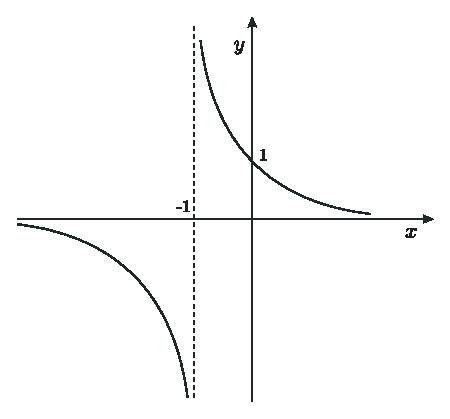
\includegraphics[width=8cm]{SL_202}
\end{center}
\end{rj}

%%\slika %0202, str. 6
%\stavisliku{eps/SL_202}


\begin{example}\label{pr 2.5}
Rije\v{s}imo diferencijalnu jednad\v{z}bu $9yy'+4x=0$.
\end{example}
\begin{rj}
Iz $9ydy=-4xdx$ integracijom nalazimo op\'{c}e rje\v{s}enje
$\displaystyle\frac{9}{2}y^2=-2x^2+\overline{c}$, tj.
$\displaystyle\frac{x^2}{9}+\frac{y^2}{4}=c$ (uz pokratu
$c=\overline{c}/18$). Op\'{c}e rje\v{s}enje predstavlja familiju
(konfokalnih) elipsa.
\end{rj}

\begin{example}\label{pr 2.6}
Rije\v{s}imo jednad\v{z}bu $y'=1+y^2$.
\end{example}
\begin{rj}
Iz $dy/(1+y)^2=dx$ integracijom nalazimo op\'{c}e rje\v{s}enje
 $$\arctg y=x+c.$$
Odavde lako nalazimo
 $$y=\tg(x+c).$$

(Primijetimo koliko je va\v{z}no odmah pri integraciji uvesti
konstantu $c$. Da smo to u\v{c}inili kasnije, dobili bismo
\textbf{pogre�no} $y=\tg x+c$.)
\end{rj}

\begin{example}\label{pr 2.7}
Rije\v{s}imo
\begin{enumerate}[\indent a)]
 \item $yy'=\cos 2x,\quad y(0)=1$;
 \item $\displaystyle\frac{dy}{dx}=\frac{x}{y+yx^2},\quad
  y(0)=-1$;
 \item $y'=x^2y^2+x^2-y^2-1,\quad y(0)=0$.
\end{enumerate}
\end{example}
\begin{rj}
%\fxnote{provjeriti jel stil rjesenja sad O.K.}
%\begin{enumerate}[\indent a)]
\mbox{}
\vspace*{-2ex}

\begin{enumerate}[a)\quad ]
\item  $\D
        y\ dy   =\cos2xdx,\quad
        \frac{y^2}{2}=\frac{1}{2}\sin2x+\overline{c},\quad y=\pm\sqrt{\sin
        2x+c}\quad
        (c=2\overline{c});$\\

        $\D y(0)   =\sqrt{\sin0+c}=1,\quad\sqrt{c}=1,\quad c=1,\quad y=\sqrt{\sin
        2x+1}.$
\item  $\D
        y \ dx   =\frac{x\,dx}{1+x^2},\quad
        \frac{y^2}{2}=\frac{1}{2}\ln(1+x^2)+\overline{c},\quad y=\pm\sqrt{\ln(1+x^2)+c}
        \quad (c=2\overline{c}); $\\

        $\D y(0)   =-\sqrt{\ln1+c}=-1,\quad -\sqrt{c}=-1,\quad c=1,\quad
        y=-\sqrt{\ln(1+x^2)+1}.       $
\item  $\D
        y' \   =(x^2-1)(y^2+1), \quad\frac{dy}{1+y^2}=(x^2-1)dx,\quad
        \arctg y=\frac{x^3}{3}-x+c,\quad$\\
        $\D
        y  =\tg\left(\frac{x^3}{3}-x+c\right);
        y(0)  =\tg(c)=0,\quad c=0, \quad $\\
        $\D
        y     =\tg\left(\frac{x^3}{3}-x\right)$
\end{enumerate}
\end{rj}

Neke od diferencijalnih jednad\v{z}bi koje smo ranije razmatrali
zapravo su separabilne. Takva je npr. jednad\v{z}ba
eksponencijalnoga rasta
 $$y'=ky.$$
Dakle, mo\v{z}emo je rije\v{s}iti ovako:
\begin{align*}
 \frac{dy}{y} & =kdx,\quad \ln|y|=kx+\overline{c}, \\
 |y| & =e^{kx+\overline{c}}=e^{kx}e^{\overline{c}},\quad y=ce^{kx},
\end{align*}
gdje je $c=+e^{\overline{c}}$ za $y>0$ i $c=-e^{\overline{c}}$ za
$y<0$. Mo\v{z}emo dopustiti i $c=0$ jer to daje trivijalno rje\v{s}enje
jednad\v{z}be eksponencijalnoga rasta $y=0$.

Jednad\v{z}ba strujnoga kruga s konstantnim naponom (primjer A iz prethodnog poglavlja)
 $$L\frac{dJ}{dt}+RJ=U$$
tako\dj{}er je separabilna, pa je mo\v{z}emo rije\v{s}iti ovako:
\begin{align*}
 L\frac{dJ}{dt} & =U-RJ,\quad \frac{L}{U-RJ}dJ=dt, \\
 \int\frac{LdJ}{U-RJ} & =\int dt+c,\quad
 -\frac{L}{R}\ln|U-RJ|=t+c, \\
 |U-RJ| & =e^{-\frac{R}{L}(t+c)},\quad U-RJ=Ae^{-\frac{R}{L}t},
\end{align*}
gdje je $\displaystyle A=\pm e^{-\frac{R}{L}c}$. Ako je $J=J_0$ u
po\v{c}etnom trenutku $t=0$, onda je $A=U-RJ_0$, pa nakon
uvr\v{s}tavanja te vrijednosti i sre\dj{}ivanja dobivenoga izraza
nalazimo rje\v{s}enje jednad\v{z}be u obliku
 $$J=\frac{U}{R}+\left(J_0-\frac{U}{R}\right)e^{-\frac{R}{L}t}.$$

U sljede\'{c}im primjerima pozabavit \'{c}emo se s jo\v{s}
nekoliko problema \v{c}iji je matemati\v{c}ki model separabilna
diferencijalna jednad\v{z}ba.

\begin{example}\label{pr 2.8}
Olovna kugla malih dimenzija zagrijana je na 100 $^\circ$C. U
trenutku $t=0$ uronimo je u vodenu kupku velikih dimenzija
\v{c}iju temperaturu konstantno odr\v{z}avamo na 30 $^\circ$C.
Toplinska vodljivost olova izuzetno je velika, pa mo\v{z}emo
pretpostaviti da je temperatura kugle jednaka u svim njezinim
to\v{c}kama u svakom pojedinom trenutku. Prema Newtonovom zakonu
hla\dj{}enja brzina promjene temperature uronjene kugle
proporcionalna je razlici temperatura kugle i vodene kupke u kojoj
se ona hladi. Na kraju tre\'{c}e minute hla\dj{}enja temperatura
kugle smanjena je na 70 $^\circ$C. Koliko \'{c}e vremena pro\'{c}i
dok se ona smanji na 31 $^\circ$C?
\end{example}
\begin{rj}
Matemati\v{c}ki model procesa hla\dj{}enja prema Newtonovom zakonu
predstavlja separabilna diferencijalna jednad\v{z}ba
 $$\frac{dT}{dt}=k(T-30).$$
Separacija varijabli i neposredna integracija dovode nas do
njezinoga op\'{c}eg rje\v{s}enja
\begin{align*}
 \frac{dT}{T-30} & =kdt,\quad \ln |T-30|=kt-\overline{c}, \\
 T(t) & =ce^{kt}+30,
\end{align*}
gdje je $c=+e^{\overline{c}}$  (jer je $T>0$). Iz po\v{c}etnog
uvjeta $T(0)=100$ odredit \'{c}emo vrijednost nepoznatog parametra
$c$:
 $$T(0)=ce^0+30=100,\quad c=70.$$
Dakle,
 $$T(t)=70e^{kt}+30.$$
Konstantu $k$ odredit \'{c}emo iz poznatog podatka da je
$T(3)=70$:
 $$T(3)=70e^{k\cdot 3}+30=70,\quad
 k=\frac{1}{3}\ln\frac{70-30}{70}=-0.1865.$$
Dakle,
 $$T(t)=70e^{-0.1865t}+30.$$
Odavde lako slijedi odgovor na na\v{s}e pitanje:
\begin{gather*}
T(t)=70e^{-0.1865t}+30=31, \\
-0.1865t=\ln(1/70),\quad t=22.78.
\end{gather*}
Temperatura \'{c}e se smanjiti na 31$^\circ$ C za ne\v{s}to manje
od 23 minute.
\end{rj}
\begin{example}\label{pr 2.9}
Padobranac otvara svoj padobran u trenutku $t=0$, kada je dosegao
brzinu $v_0$. Njegovu masu, zajedno s opremom, ozna\v{c}imo s $m$.
Otpor kojim se zrak opire njegovom padu proporcionalan je kvadratu
brzine, $F_{otp}=kv^2$ (konstanta $k$ ovisi o veli\v{c}ini i
obliku padobrana). Kako se mijenja brzina padobranca ovisno o
vremenu proteklom nakon otvaranja padobrana?
\end{example}
\begin{rj}
Prema drugom Newtonovom zakonu
 $$F=ma=m\frac{dv}{dt},$$
No, ukupna sila $F$ koja djeluje na padobranca jednaka je razlici
sile   te\v{z}ine $mg$ i njoj suprotno
usmjerene sile otpora $F_{otp}=kv^2$. Dakle,
 $$mg-kv^2=m\frac{dv}{dt},$$
odnosno, nakon dijeljenja s $m$ i uz pokratu $b^2=mg/k$,
 $$\frac{dv}{dt}=-\frac{k}{m}(v^2-b^2).$$
Ova separabilna diferencijalna jednad\v{z}ba matemati\v{c}ki je
model na\v{s}ega problema. Rije\v{s}imo je.
\begin{align*}
 \frac{dv}{v^2-b^2} & =-\frac{k}{m}\ dt, \\
 \int\frac{dv}{v^2-b^2} & =-\frac{k}{m}t+\overline{c}.
\end{align*}
Iz poznatog nam rastava na parcijalne razlomke
 $$\frac{1}{v^2-b^2}=\frac{1}{2b}\left(\frac{1}{v-b}-\frac{1}{v+b}\right)$$
lako nalazimo
 $$\int\frac{dv}{v^2-b^2}=\frac{1}{2b}\ln\left|\frac{v-b}{v+b}\right|=-\frac{k}{m}t+\overline{c}.$$
Uz pokratu $p=2kb/m$ slijedi
 $$\frac{v-b}{v+b}=ce^{-pt},$$
gdje je $c=+e^{2b\overline{c}}$ ili $c=-e^{2b\overline{c}}$ ovisno
o tome je li gornji razlomak pozitivan ili negativan.
Uvr\v{s}tavanjem po\v{c}etnog uvjeta $v(0)=v_0$ u gornju
jednad\v{z}bu, nalazimo da je $c=(v_0-b)/(v_0+b)$. Rije\v{s}imo li
gornju jednad\v{z}bu po $v$, na\'{c}i \'{c}emo
 $$v(t)=b\frac{1+ce^{-pt}}{1-ce^{-pt}},$$
gdje je $b=\sqrt{mg/k}$, $p=2\sqrt{kg/m}$ i
$c=(v_0-\sqrt{mg/k})/(v_0+\sqrt{mg/k})$ . Primijetimo da je
$\displaystyle\lim_{t\to\infty} v(t)=b=\sqrt{mg/k}$. To zna\v{c}i
da se brzina padobranca nakon otvaranja padobrana smanjuje,
te\v{z}e\'{c}i prema grani\v{c}noj vrijednosti $\sqrt{mg/k}$ koja
ne ovisi (!) o brzini $v_0$ pri kojoj je otvoren padobran. Dva
tipi\v{c}na grafa brzine $v(t)$, za $v_0>\sqrt{mg/k}$ i
$v_0<\sqrt{mg/k}$, prikazana su na sljede\'coj slici
%\slika %0203, str. 11.

\stavisliku{eps/SL_203}
\end{rj}

\begin{example}\label{pr 2.10}
Odredimo ravnote\v{z}ni oblik koji u polju sile te\v{z}e poprima
na dva kraja obje\v{s}eni lanac specifi�ne duljinske mase $m$ ( za koji
pretpostavljamo da je idealno savitljiv). Krivulju toga oblika
zovemo lan\v{c}anicom\index{lan�anica}.
\end{example}
\begin{rj}
Lanac o\v{c}ito le\v{z}i u vertikalnoj ravnini i osno je
simetri\v{c}an u odnosu na vertikalu koja prolazi njegovom
najni\v{z}om to\v{c}kom. Promotrimo desnu polovicu lan\v{c}anice:

%\slika %0204, str. 11.
\stavisliku{eps/SL_204_V1}

Sila napetosti lanca $T$ mora izbalansirati horizontalnu silu
napetosti $H$ i vertikalnu te\v{z}inu lanca $m gs$, gdje je $s$
duljina lanca od najni\v{z}e to\v{c}ke, u kojoj djeluje $H$, do
to\v{c}ke u kojoj djeluje $T$. Dakle,
\begin{align*}
 T\cos\vartheta & = H, \\
 T\sin\vartheta & =m gs,
\end{align*}
odakle dijeljenjem dobivamo
 $$\frac{T\sin\vartheta}{T\cos\vartheta}=\tg\vartheta=\frac{m g}{H}s.$$
S druge strane, $tg\vartheta$ nagib je lan�anice $y=y(x)$, tj.
$\displaystyle\tg\vartheta=\frac{dy}{dx}$. Slijedi da
lan\v{c}anica zadovoljava jednad\v{z}bu
 $$\frac{dy}{dx}=\frac{mg}{H}s.$$
Budu\'{c}i da je
 $$\frac{ds}{dx}=\sqrt{\frac{dx^2+dy^2}{dx^2}}=\sqrt{1+\left(\frac{dy}{dx}\right)^2},$$
slijedi da lan\v{c}anica $y=y(x)$ zadovoljava diferencijalnu
jednad\v{z}bu
 $$\frac{d^2y}{dx^2}=\frac{mg}{H}\frac{ds}{dx}=\frac{mg}{H}\sqrt{1+\left(\frac{dy}{dx}\right)^2}.$$
To je diferencijalna jednad\v{z}ba drugoga reda za $y$, ali prvoga
reda (i to separabilna) za $\displaystyle u=\frac{dy}{dx}$:
\begin{gather*}
 \frac{du}{dx}  =\frac{mg}{H}\sqrt{1+u^2}, \\
 \frac{du}{\sqrt{1+u^2}}  =\frac{mg}{H}dx,
\end{gather*}
\v{c}ije je rje\v{s}enje
 $$\Arsh u=\frac{mg}{H}x+c.$$
Lan\v{c}anica je horizontalna za $x=0$, tj.
$\displaystyle\frac{dy}{dx}(0)=u(0)=0$, \v{s}to zna\v{c}i da je
$c=0$. Dakle, \FIXME{pogl. 2, str. 12, srediti formulu}
\begin{gather*}
 \Arsh u=\frac{mg}{H}x,\quad u=\sh\frac{mg}{H}x, \\
 u=\frac{dy}{dx}=\sh\frac{mg}{H}x,\quad
 y=\frac{H}{mg}ch\frac{mg}{H}x.
\end{gather*}
Lan\v{c}anica je graf dobro nam poznatog kosinusa hiperbolnog.
\end{rj}

Neke diferencijalne jednad\v{z}be, iako nisu separabilne, mogu to
postati primjenom jednostavnih supstitucija. Takve su sve
jednad\v{z}be oblika
 $$y'=f\left(\frac{y}{x}\right),$$
gdje je $f$ proizvoljna funkcija od $y/x$, npr. $(y/x)^2$,
$\sin(y/x)$, $e^{y/x}$, itd. Uvedemo li supstituciju
 $$\frac{y}{x}=u,\quad \text{ tj. }\quad y=xu,$$
slijedi da je
 $$y'=u+xu',$$
pa na\v{s}a polazna jednad\v{z}ba prelazi u separabilnu
jednad\v{z}bu
\begin{align*}
 u+xu' & =f(u), \\
 \frac{du}{f(u)-u} & =\frac{dx}{x}.
\end{align*}
Nju rje\v{s}avamo na poznati na\v{c}in, a kada na\dj{}emo funkciju
$u$, uvrstimo je u jednad\v{z}bu na\v{s}e supstitucije, $y=xu$, i
tako na\dj{}emo tra\v{z}enu funkciju $y$. Evo jednog konkretnog
primjera.

\begin{example}\label{pr 2.11}
Rije�imo jednad�bu $2xyy'-y^2+x^2=0$.
\end{example}
\begin{rj}
Dijeljenjem s $x^2$ dobijemo
 $$2\frac{y}{x}y'-\left(\frac{y}{x}\right)^2+1=0.$$
Uz supstituciju $y=xu$, $y'=u+xu'$ jednad\v{z}ba prelazi u
separabilnu jednad\v{z}bu
 $$2u(u+xu')-u^2+1=0.$$
Rije\v{s}imo je za $u$:
$$\begin{array}{rl}
 \displaystyle 2xu\frac{du}{dx}+u^2+1=0, & \quad \displaystyle\frac{2udu}{1+u^2}=-\frac{dx}{x},
 \\
 \displaystyle\ln(1+u^2)=-\ln x+\overline{c}, & \displaystyle\quad \ln(1+u^2)=\ln\frac{c}{x},
 \\
 \displaystyle 1+u^2=\frac{c}{x},
\end{array}$$
gdje je $c=e^{\overline{c}}$. Uvr\v{s}tavanjem $\displaystyle
u=\frac{y}{x}$ dolazimo do (implicitno zadanog) op\'{c}eg
rje\v{s}enja polazne jednad\v{z}be: \FIXME{pogl 2, str. 14,
srediti formulu}
\begin{gather*}
 1+\frac{y^2}{x^2}=\frac{c}{x},\quad x^2+y^2=cx, \\
 \left(x-\frac{c}{2}\right)^2+y^2=\frac{c^2}{4}.
\end{gather*}
Op\'{c}e rje\v{s}enje predstavlja familiju kru\v{z}nica kojima je
sredi\v{s}te na osi $x$, a sve prolaze ishodi\v{s}tem.
\begin{center}
  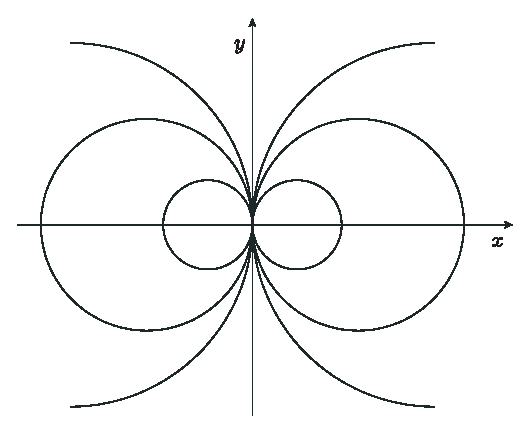
\includegraphics{SL_205}
\end{center}
\end{rj}

Oblik diferencijalne jednad\v{z}be katkada sugerira neku drugu
jednostavnu supstituciju, \v{s}to ilustrira sljede\'{c}i primjer.
\begin{example}\label{pr 2.12}
Rije\v{s}imo jednad\v{z}bu
 $$(2x-4y+5)y'+x-2y+3=0.$$
\end{example}
\begin{rj}
Supstituiramo li $x-2y=v$, slijedi $\displaystyle
y'=\frac{1}{2}(1-v')$, \v{s}to dovodi do separabilne jednad\v{z}be
koju lako rje\v{s}avamo: \FIXME{pogl. 2, str. 15, srediti formulu}
\begin{gather*}
 (2v+5)\frac{1}{2}(1-v')+v+3=0, \\
 4v+11=(2v+5)v', \\
 \frac{2v+5}{4v+11}\ dv=dx,\quad\frac{4v+10}{4v+11}\ dv=2\ dx, \\
 \left(1-\frac{1}{4v+11}\right)dv=2 \ dx, \\
 v-\frac{1}{4}\ln|4v+11|=2x+\overline{c}.
\end{gather*}
Uvr\v{s}tavanjem $v=x-2y$ nalazimo op\'{c}e (implicitno)
rje\v{s}enje polazne jednad\v{z}be,
 $$4x+8y+\ln|4x-8y+11|=c.$$
\end{rj}

Separabilne diferencijalne jednad\v{z}be uspijevamo rje\v{s}iti
obi\v{c}nom integracijom. Rje\v{s}avanje nekih drugih tipova
diferencijalnih jednad\v{z}bi mo\v{z}e se svesti na obi\v{c}nu
integraciju upotrebom odgovaraju\'{c}ih transformacija. Sada
\'{c}emo se pozabaviti takvim tipom jednad\v{z}bi.

Diferencijalnu jednad\v{z}bu zovemo linearnom ako predstavlja
linearnu vezu nepoznate funkcije $y$ i njezinih derivacija, s
koeficijentima koji su zadane funkcije od $x$. Dakle, linearna
diferencijalna jednad\v{z}ba prvoga reda ima oblik
\begin{equation}\label{eq 2.3}
 y'+p(x)y=q(x),
\end{equation}
gdje su $p(x)$ i $q(x)$ zadane funkcije.

Pomno\v{z}imo jednad\v{z}bu \eqref{eq 2.3} zasad jo\v{s}
neodre\dj{}enom funkcijom $z=z(x)$:
 $$y'z+p(x)yz=q(x)z.$$
Lijeva strana dobivene jednad\v{z}be bit \'{c}e integrabilna ako
je
 $$y'z+yp(x)z=\frac{d}{dx}(yz)=y'z+yz',$$
tj. ako je $p(x)z=z'$. No ta je jednad\v{z}ba separabilna, pa lako
nalazimo jedan takav integriraju\'{c}i faktor $z$:
\begin{align*}
 \frac{dz}{dx} & =p(x)z,\quad\frac{dz}{z}=p(x)dx, \\
 \ln|z| & =\int p(x)dx,\quad z=e^{P(x)},
\end{align*}
gdje je $P(x)=\int p(x)dx$. Uvrstimo li integriraju\'{c}i faktor
$z=e^{P(x)}$ u po\v{c}etnu jednad\v{z}bu, dobivamo \FIXME{pogl. 2,
str 16, srediti formulu}
\begin{gather*}
 y'e^{P(x)}+yp(x)e^{P(x)} = q(x)e^{P(x)} \\
 \frac{d}{dx}\left(ye^{P(x)}\right) = q(x)e^{P(x)}, \\
 ye^{P(x)} = c+\int q(x)e^{P(x)}dx, \\
 y = e^{-P(x)}\left(c+\int q(x)e^{P(x)}dx\right),
\end{gather*}
gdje je $c$ proizvoljna konstanta integracije.



\plavapozadina{
\begin{okvir}[Linearna diferencijalna jednad\v{z}ba]
\index{linearna diferencijalna jednad�ba}
\index{diferencijalna jednad�ba!linearna}
  Linearnu jednad\v{z}bu oblika
 $$y'+p(x)y=q(x)$$
rje\v{s}avamo na sljede\'{c}i na\v{c}in:
\begin{enumerate}
 \item Izra\v{c}unamo integriraju\'{c}i faktor $z$\index{integriraju�i faktor}
  $$z=e^{P(x)},\quad P(x)=\int p(x)dx.$$
 \item Pomno\v{z}imo jednad\v{z}bu s tim faktorom i zatim integriramo,
       koriste\'{c}i se \v{c}injenicom da je integral lijeve strane
       \textbf{uvijek} $ye^{P(x)}$. \\ Dobiveno je op\'{c}e
       rje\v{s}enje
       $$y=e^{-P(x)}\left(c+\int q(x)e^{P(x)}dx\right).$$
 \item Partikularno rje\v{s}enje, koje zadovoljava po\v{c}etni uvjet $y(x_0)=y_0$,
       nalazimo uvr\v{s}tavanjem toga uvjeta u op\'{c}e rje\v{s}enje.
\end{enumerate}
\end{okvir}}


\begin{example}\label{pr 2.13}
Rije\v{s}imo linearnu diferencijalnu jednad\v{z}bu
 $$y'+xy=x,$$
uz po\v{c}etni uvjet $y(0)=3.$
\end{example}

\fxnote{prijelom}

\newpage
\begin{rj}
 \begin{enumerate}
  \item Na\dj{}imo integriraju\'{c}i faktor $z$:
         \begin{align*}
          P(x) & =\int p(x)dx=\int xdx=\frac{x^2}{2}, \\
          z & = e^{x^2/2.}
         \end{align*}
  \item Pomno\v{z}imo jednad\v{z}bu s tim faktorom:
       \begin{align*}
        y'e^{x^2/2}+yxe^{x^2/2} & = xe^{x^2/2}, \\
        \frac{d}{dx}\left(ye^{x^2/2}\right) & =xe^{x^2/2},
       \end{align*}
       pa zatim integriramo
       $$ye^{x^2/2}=\int xe^{x^2/2}dx=e^{x^2/2}+c.$$
       Slijedi da je op\'{c}e rje\v{s}enje na\v{s}e jednad\v{z}be
        $$y=1+ce^{-x^2/2}.$$
 \item Iz po\v{c}etnog uvjeta, $y(0)=3$, uvr\v{s}tavanjem slijedi
       $$y(0)=1+c=3,\quad c=2,$$
       pa je tra\v{z}eno partikularno rje\v{s}enje
       $$y=1+2e^{-x^2/2}.$$
 \end{enumerate}
\end{rj}

Neke diferencijalne jednad\v{z}be, koje smo rije\v{s}ili drugim
metodama, linearne su, pa ih sada mo\v{z}emo rije\v{s}iti kao
takve. Na primjer, jednad\v{z}ba $RL$-strujnoga kruga s
izmjeni\v{c}nim naponom (primjer A
%\fxnote{pogl. 2, str. 18, ref na pr}
 iz prethodnog poglavlja)
 $$L\frac{dJ}{dt}+RJ=U_0\cos\omega t,$$
linearna je. Napi\v{s}emo li je u obliku
 $$\frac{dJ}{dt}+\frac{R}{L}J=\frac{U_0}{L}\cos\omega t,$$
vidimo da je u tom slu\v{c}aju $\displaystyle p(t)=\frac{R}{L}$,
tj. $\displaystyle P(t)=\frac{R}{L}t$ i $\displaystyle
q(t)=\frac{U_0}{L}\cos\omega t$, pa je njezino op\'{c}e
rje\v{s}enje
 $$J=e^{-\frac{R}{L}t}\left(c+\frac{U_0}{L}\int \cos\omega
 te^{\frac{R}{L}t}dt\right).$$
Dvostrukom parcijalnom integracijom mo\v{z}emo izra\v{c}unati
 $$\int\cos\omega te^{\frac{R}{L}t}dt=\frac{Le^{\frac{R}{L}t}}{R^2+L^2\omega^2}
   (R\cos\omega t+L\omega\sin\omega t),$$
odakle slijedi
 $$J=\frac{U_0}{R^2+L^2\omega^2}(R\cos\omega t+L\omega\sin\omega
 t)+ce^{-\frac{R}{L}t},$$
odnosno, uz $\vartheta =\arctg L\omega/R$ (prema pravilu za
superponiranja oscilacije iste frekvencije),
 $$J=\frac{U_0}{\sqrt{R^2+L^2\omega^2}}\cos (\omega
 t-\vartheta)+ce^{-\frac{R}{L}t}.$$

Vrijednost konstante $c$ odre\dj{}ena je jako\v{s}\'{c}u struje
$J$ u trenutku $t=0$. Primijetimo da $J$ sadr\v{z}i oscilatorni,
stacionarni dio, \v{c}ija je frekvencija $\omega$ jednaka
frekvenciji izvora kojim se napaja strujni krug (usp.~primjer
\FIXME{pogl. 2, str. 18, ref na pr} u prethodnom poglavlju) i
prelazni, nestacionarni dio $\displaystyle ce^{-\frac{R}{L}t}$
koji s vremenom nestaje.

%\slika %0206, str. 19.
%\stavisliku{SL_206.eps}
\begin{center}
  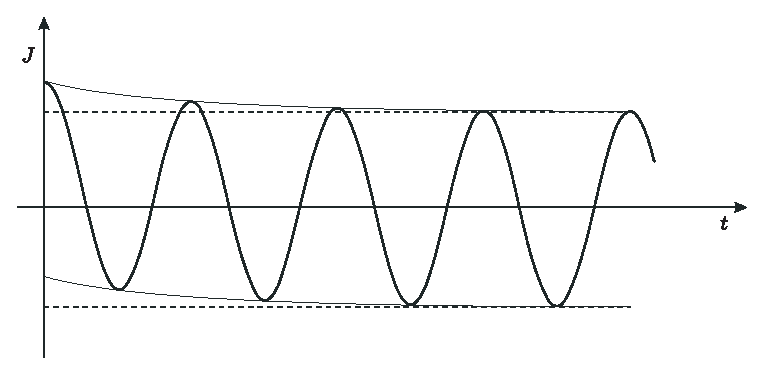
\includegraphics[width=12cm]{SL_206}
\end{center}

Ako je $c=0$, dobivamo partikularno stacionarno rje\v{s}enje, koje
smo na\v{s}li u prethodnom odjeljku, prijelazom u kompleksno
podru\v{c}je. Oscilacija struje i napona bit \'{c}e u fazi ako je
$\vartheta =\arctg L\omega/R=0$, tj. ako je $L=0$.

Linearna diferencijalna jednad\v{z}ba modelira i $RC$-strujni
krug\index{RCstrujni@$RC$-strujni krug},
s otpornikom otpora $R$ i kondenzatorom kapaciteta $C$.


\begin{center}
  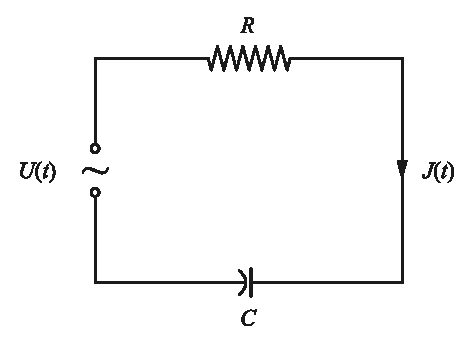
\includegraphics[width=7cm]{SL_207}
\end{center}

Ve\'{c} smo spomenuli da je pad napona du\v{z} otpornika
proporcionalan trenutnoj struji $J$ (Ohmov zakon)
 $$U_R=RJ,$$
a eksperimentalno se tako\dj{}er pokazuje da je pad napona na
kondenzatoru proporcionalan trenutnom naboju $Q$ kondenzatora
 $$U_C=\frac{1}{C}Q,$$
gdje je $C$ kapacitet kondenzatora. Budu\'{c}i da je
$\displaystyle J(t)=\frac{dQ}{dt}$, to mo\v{z}emo zapisati i u
obliku
 $$U_C=\frac{1}{C}\int J(t)dt,$$
pa iz drugog Kirchhoffovog zakona (o naponima) slijedi
 $$U=RJ+\frac{1}{C}\int J(t)dt.$$
Nakon deriviranja lijeve i desne strane dobivamo linearnu
diferencijalnu jednad\v{z}bu $RC$ - kruga:
 $$\begin{array}{r@{\,}c@{\,}l}
    \displaystyle\frac{dU}{dt} &\displaystyle = R\frac{dJ}{dt}+\frac{1}{C}J, \\[2ex]
    \displaystyle\frac{dJ}{dt} &\displaystyle +\frac{1}{RC}J=\frac{1}{R}\frac{dU}{dt}.
   \end{array}$$
u kojoj je $p(t)=1/RC$, tj. $P(t)=t/RC$ i $q(t)=(1/R)dU/dt$.

Njezino op\'{c}e rje\v{s}enje je
 $$J(t)=e^{-\frac{t}{RC}}\left(K+\frac{1}{R}\int
 e^{\frac{t}{RC}}\frac{dU}{dt}dt\right).$$
Konstantu integracije ozna\v{c}ili smo s $K$ da je razlikujemo od
kapaciteta $C$. Ako je strujni krug priklju\v{c}en na izvor
konstantnog napona $U$, onda je $\displaystyle\frac{dU}{dt}=0$, pa
je jakost struje u tom slu\v{c}aju
 $$J(t)=Ke^{-\frac{t}{RC}}.$$

%\slika %0208, str. 21.
\stavisliku{eps/SL_208}

Ako je strujni krug priklju\v{c}en na izvor izmjeni\v{c}nog napona
$U(t)=U_0\sin\omega t$, onda je
$\displaystyle\frac{dU}{dt}=\omega U_0\cos\omega t$, pa je jakost struje
u tom slu\v{c}aju
\begin{align*}
 J(t) & =Ke^{-\frac{t}{RC}}+\frac{\omega U_0C}{1+\omega^2R^2C^2}(\cos\omega t+\omega RC\sin\omega
 t)= \\
 & = Ke^{-\frac{t}{RC}}+\frac{\omega
 U_0C}{\sqrt{1+\omega^2R^2C^2}}\cos (\omega t+\vartheta),
\end{align*}
gdje je $\vartheta=\arctg\omega RC$ (prema pravilu za
superponiranje oscilacija). Jakost struje $J$ opet se sastoji od
stacionarnog dijela frekvencije $\omega$ i nestacionarnog dijela
$\displaystyle Ke^{-\frac{t}{RC}}$, koji s vremenom nestaje.

$RLC$ - strujni krugovi\index{RLCstrujni@$RLC$-strujni krugovi} koji sadr\v{z}e sve tri komponente, otpornik,
induktor i kondenzator, matemati\v{c}ki se modeliraju linearnom
diferencijalnom jednad\v{z}bom drugoga reda. Naime, iz drugog
Kirchhoffova zakona (o naponima) slijedi
 $$RJ+L\frac{dJ}{dt}+\frac{1}{C}\int J(t)dt=U,$$
pa deriviranjem dobivamo linearnu jednad\v{z}bu drugog reda
 $$L\frac{d^2J}{dt^2}+R\frac{dJ}{dt}+\frac{1}{C}J=\frac{dU}{dt}.$$
Takve \'{c}emo jednad\v{z}be rje\v{s}avati u sljede\'{c}em
poglavlju.

U primjerima \ref{pr 2.14}, \ref{pr 2.15} i \ref{pr 2.16}  pozabavit
\'{c}emo se s jo\v{s} nekoliko problema \v{c}iji je
matemati\v{c}ki model linearna diferencijalna jednad\v{z}ba prvoga
reda.

\begin{example}\label{pr 2.14}
Sila te\v{z}e, koja djeluje na tijelo mase $m$ \v{s}to slobodno
pada kroz zrak, iznosi $mg$, gdje je $g$ gravitacijska konstanta.
Pretpostavit \'{c}emo da je sila kojom se zrak opire padu
proporcionalna $\vartheta$ brzini tijela, $\gamma v$, gdje je
$\gamma$ konstanta proporcionalnosti. Na\dj{}imo ovisnost brzine
tijela o vremenu $t$ (prije no \v{s}to tijelo udari u tlo).
\end{example}
\begin{rj}
Iz drugog Newtonovog zakona slijedi
 $$\begin{array}{r@{\,}l@{\,}c}
  \displaystyle ma & \displaystyle =m\frac{dv}{dt}=mg-\gamma v, \\
  \displaystyle\frac{dv}{dt} & \displaystyle+\frac{\gamma}{m}v=g,
 \end{array}$$
\v{s}to je linearna jednad\v{z}ba s $p(t)=\gamma/m$, $P(t)=\gamma
t/m$ i $q(t)=g$, pa je njezino rje\v{s}enje
 \begin{align*}
  v(t) & =e^{-\gamma t/m}\left(K+\int ge^{\gamma t/m}dt\right)= \\
       & =e^{-\gamma t/m}\left(K+\frac{mg}{\gamma}e^{\gamma
       t/m}\right).
 \end{align*}
Ako je $v=0$ u trenutku ispu\v{s}tanja $t=0$, onda je
$K=-mg/\gamma$, pa je
 $$v(t)=\frac{mg}{\gamma}(1-e^{-\gamma t/m}).$$
Za $t\to\infty$, $e^{-\gamma t/m}\to 0$, \v{s}to zna\v{c}i da je
brzina tijela ome�ena grani\v{c}nom brzinom $mg/\gamma$.
\begin{center}
\setlength\unitlength{1mm}
%\fbox
{\begin{picture}(85,35)
\put( 8,20){\small $\frac{mg}{\gamma}$}
\put(27.5,25.5){\small$v=gt$}
\put(10,0){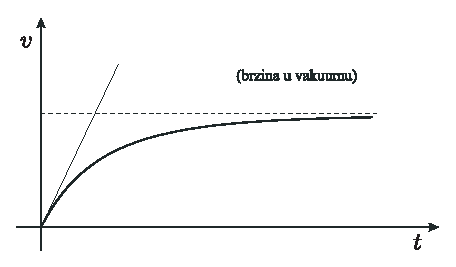
\includegraphics{SL_209}}
\end{picture}}
\end{center}
Za male $t$ vrijedi $e^{-\gamma t/m}\approx 1-\gamma t/m$. Tada je
$v(t)\approx gt$, \v{s}to je iznos brzine u vakuumu (dakle, bez otpora
zraka). Kako $t$ raste, otpor zraka usporava rast brzine tijela do
grani\v{c}ne brzine $mg/\gamma$.
\end{rj}

Ne\v{s}to op\'{c}enitiji od prethodnog problema jest problem
kosoga hica u mediju\index{kosi hitac!u mediju} koji se opire gibanju projektila (npr.~u
zraku).

\begin{example}\label{pr 2.15}
 Na\dj{}imo parametarske jednad\v{z}be gibanja projektila u polju sile te\v{z}e
 (kroz zrak koji se opire gibanju silom koja je proporcionalna brzini gibanja).
\end{example}
\begin{rj}
Projektil se giba u vertikalnoj ravnini $xy$. Pretpostavimo da
je iz po\v{c}etnog polo\v{z}aja (0,0) ispaljen brzinom $v_0$ pod
kutom $\alpha$.

%\slika %0210, str. 23
%\stavisliku{SL_210}
%\fxnote{ma i ova slika je gadna, premala?}
\begin{center}
  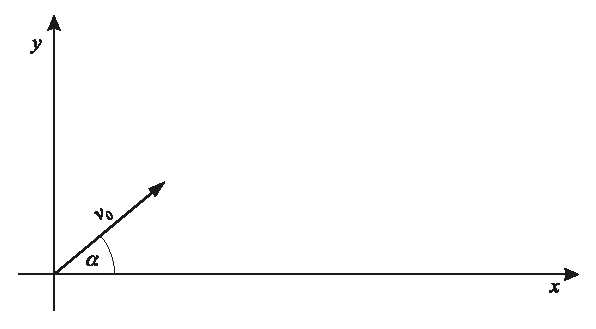
\includegraphics[width=11cm]{SL_210}
\end{center}


U horizontalnom smjeru $x$ na projektil djeluje samo sila
zra\v{c}noga otpora, koja je proporcionalna brzini, pa je prema
drugom Newtonovom zakonu
 $$m\ddot{x}=-K\dot{x},\quad \ddot{x}=-k\dot{x},\quad (k=K/m).$$
U vertikalnom smjeru $y$ na projektil djeluje sila te\v{z}e i sila
otpora, pa je
 $$m\ddot{y}=-mg-K\dot{y},\quad \ddot{y}=-g-k\dot{y}\quad(k=K/m).$$
(minus $mg$, jer je $y$ os usmjerena \textbf{gore}, u smjeru
suprotnom sili te\v{z}e).

Prva, $x$-jednad\v{z}ba, linearna je za $v_x=\dot{x}$
($\dot{v}_x=-kv_x$) i njezino nam je rje\v{s}enje dobro poznato:
 $$\dot{x}=v_x=Ce^{-kt}.$$
Iz po\v{c}etnog uvjeta $v_x(0)=v_0\cos\alpha$ slijedi
$C=v_0\cos\alpha$, pa je
 $$\dot{x}=v_x=v_0\cos\alpha e^{-kt}.$$
Integracijom nalazimo
 $$x=-\frac{v_0\cos\alpha}{k}e^{-kt}+D,$$
a iz po�etnog uvjeta $x(0)=0$ slijedi $D=v_0\cos\alpha/k$, tj.
\begin{equation}\tag{$i$}\label{eq 2.i}
 x=\frac{v_0\cos\alpha}{k}(1-e^{-kt})
\end{equation}
Druga, $y$-jednad\v{z}ba, linearna je za $\dot{y}=v_y$,
$\dot{v}_y+kv_y=-g$ i njezino je rje\v{s}enje
 $$\dot{y}=v_y=\frac{1}{k}(Ce^{-kt}-g).$$
Iz po\v{c}etnog uvjeta $v_y(0)=v_0\sin\alpha$ slijedi
$C=kv_0\sin\alpha+g$ pa je
 $$\dot{y}=v_y=v_0\sin\alpha
 e^{-kt}+\frac{g}{k}e^{-kt}-\frac{g}{k}.$$
Integracijom nalazimo
 $$y=-\frac{v_0\sin\alpha}{k}e^{-kt}-\frac{g}{k^2}e^{-kt}-\frac{gt}{k}+D.$$
Iz po\v{c}etnog uvjeta $y(0)=0$ slijedi
 $$D=(v_0\sin\alpha/k)+(g/k^2),$$
tj.
\begin{equation}\tag{$ii$}\label{eq 2.ii}
 y=-\frac{gt}{k}+\left(\frac{v_0\sin\alpha}{k}+\frac{g}{k^2}\right)(1-e^{-kt}).
\end{equation}

Graf putanje projektila, koji je odre\dj{}en parametarskim
jednad\v{z}bama putanje \eqref{eq 2.i} i \eqref{eq 2.ii}, dan je
na sljede�oj slici. Radi usporedbe
dan je i graf paraboli\v{c}ne putanje u vakuumu (usp.~primjer~B
 u prethodnom poglavlju).

%\slika %0211, str. 23
\fxnote{ovu sliku (211) bi bilo dobro uskladiti s prethodnom (210)}
\begin{center}
  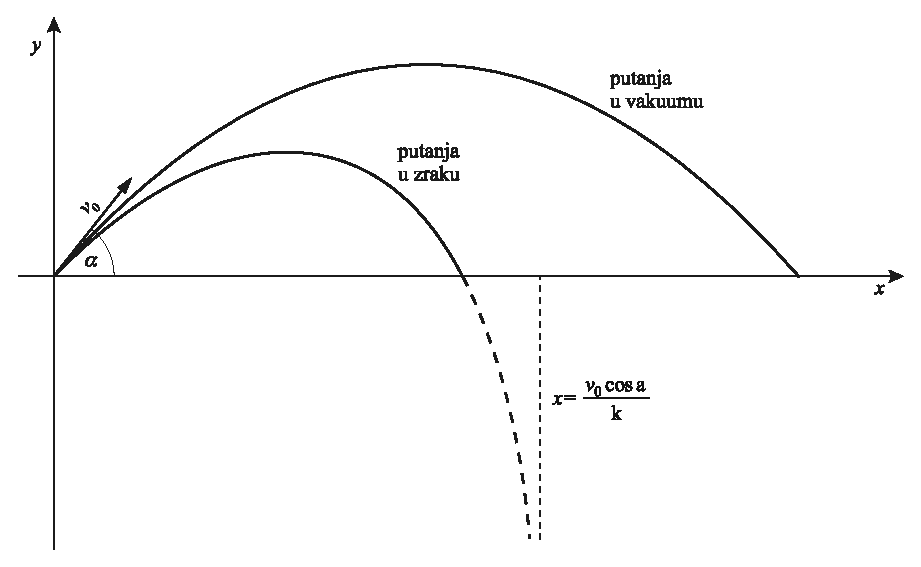
\includegraphics[width=13cm]{SL_211}
\end{center}

U prvom dijelu putanja u zraku polo\v{z}enija je od putanje u
vakuumu, dok je u drugom dijelu strmija od one u vakuumu.
Projektil udara u zemlju pod o\v{s}trijim kutom i s manjom brzinom
od one pod kojom je ispaljen. Variranjem kuta ispaljivanja lako
bismo ustanovili da se uz zadanu po\v{c}etnu brzinu maksimalni
doseg projektila posti\v{z}e uz kut ispaljivanja manji od
45$^\circ$ (\v{s}to je kut maksimalnog dosega u vakuumu).
\end{rj}
\begin{example}\label{pr 2.16}
Bure po\v{c}etno sadr�i 100 l vode u kojoj je otopljeno 50 dag
soli. U njega brzinom od 10 l/min utje\v{c}e slana voda s
koncentracijom 2 dag/l, ali voda iz njega i istje\v{c}e jednakom
brzinom. (Mije\v{s}anjem se odr\v{z}ava jednolika koncentracija
soli u buretu.) Na\dj{}imo kako se koncentracija soli u buretu
mijenja s vremenom.
\end{example}
\begin{rj}
Trenutnu koli\v{c}inu soli u buretu ozna\v{c}imo s $y(t)$. Brzina
kojom se ona mijenja jednaka je brzini ulaza soli, $10\cdot 2=20$
dag/min, umanjenoj za brzinu izlaza soli, $(10/100)y=0.1y$ dag/min
($y$ je ukupna koli\v{c}ina soli u buretu, a 10/100 dio je slane
vode koji izlazi iz bureta u jednoj minuti). Dakle,
 $$y'=20-0.1 y,$$
uz po\v{c}etni uvjet
 $$y(0)=50.$$
Op\'{c}e rje\v{s}enje linearne jednad\v{z}be koja modelira na\v{s}
problem glasi:
 \begin{align*}
  y & = e^{-0.1t}\left(C+\int e^{0.1t}20 dt\right) = \\
    & = e^{-0.1t}\left(C+\frac{20}{0.1}e^{0.1t}\right) = \\
    & =Ce^{-0.1t}+200.
 \end{align*}
Uvr\v{s}tavanjem po\v{c}etnog uvjeta nalazimo
 $$y(0)=C+200=50,\quad C=-150,$$
pa je trenutna koli\v{c}ina soli u buretu
 $$y(t)=200-150 e^{-0.1t}\text{ dag }.$$
Koncentraciju $\gamma(t)$ dobijemo dijeljenjem sa 100
(koli\v{c}ina je vode u buretu 100 l):
 $$\gamma(t)=2-1.5 e^{-0.1t} \text{ dag/l}.$$
Vidimo da koncentracija soli u buretu monotono raste prema
koncentraciji soli u vodi koja ulazi u bure, \v{s}to i
o\v{c}ekujemo.
\end{rj}

Neke nelinearne diferencijalne jednad\v{z}be mogu se svesti na
linearne. Najpoznatija je me\dj{}u njima Bernoullijeva
jednad\v{z}ba\index{diferencijalna jednad�ba!Bernoullijeva}
\begin{equation}\label{eq 2.4}
 y'=p(x)y+q(x)y^a,
\end{equation}
gdje je eksponent $a$ bilo koji realan broj. Ako je $a=0$ ili
$a=1$, jednad\v{z}ba je linearna. Ako nije, uvodimo supstituciju
 $$u=y^{1-a}.$$
Deriviranjem i uvr\v{s}tavanjem $y'$ iz \eqref{eq 2.4} dolazimo do
linearne jednad\v{z}be za $u$:
 \begin{align*}
  u' & =(1-a)y^{-a}y'=(1-a)y^{-a}(py+qy^a)= \\
     & =(1-a)(py^{1-a}+q)=(1-a)(pu+q), \\
  u' & =(1-a)pu+(1-a)q.
 \end{align*}
Ovu jednad\v{z}bu rije\v{s}imo na uobi\v{c}ajeni na\v{c}in, pa
kada smo na\v{s}li $u$, lako nalazimo i $y$ iz $u=y^{1-a}$.


\plavapozadina{
\begin{okvir}[Bernoullijeva jednad\v{z}ba]
\index{diferencijalna jednad�ba!Bernoullijeva}
\index{Bernoullijeva jednad�ba}
Bernoullijeva jednad\v{z}ba, oblika
 $$y'=p(x)y+q(x)y^a,$$
svodi se supstitucijom $u=y^{1-a}$ na linearnu jednad\v{z}bu za
$u$.
\end{okvir}}


\begin{example}\label{pr 2.17}
Rije\v{s}imo Bernoullijevu jednad\v{z}bu
 $$y'=y+y^2.$$
\end{example}
\begin{rj}
Supstitucija $u=y^{1-2}=y^{-1}$ daje
 \begin{align*}
  u' & =-y^{-2}y'=-y^{-2}(y+y^2)=-y^{-1}-1=-u-1, \\
  u' & =-u-1
 \end{align*}
Rje\v{s}enje je ove linearne jednad\v{z}be
 $$u=e^{-x}\left(C-\int e^x\,dx\right)=Ce^{-x}-1.$$
Iz $u=y^{-1}$ slijedi $y=u^{-1}=1/u$, pa je tra\v{z}eno op\'{c}e
rje\v{s}enje zadane Bernoullijeve jednad\v{z}be
 $$y=\frac{1}{1-Ce^{-x}}.$$
\end{rj}
\begin{example}\label{pr 2.18}
Mnoge populacije rastu po tzv.~logisti\v{c}kom zakonu\index{logisti�ki zakon}; brzina
rasta populacije proporcionalna je veli\v{c}ini same populacije
(npr.~zbog razmno\v{z}avanja), dok je brzina njezinoga opadanja
proporcionalna kvadratu njezine veli\v{c}ine (npr.~zbog smrtnosti
uvjetovane ograni\v{c}enim koli\v{c}inama hrane). Dakle,
 $$y'=Ay-By^2,$$
\v{s}to je Bernoullijeva jednad\v{z}ba. Izra\v{c}unajmo kakav je
rast populacije po logisti\v{c}kom zakonu.
\end{example}
\begin{rj}
Uvedemo li supstituciju $u=y^{1-2}=y^{-1}$, Bernoullijeva
jednad\v{z}ba za $y$ svodi se na linearnu za $u$:
 \begin{align*}
  u' & =-y^{-2}y'=-y^{-2}(Ay-By^2)=B-Ay^{-1}, \\
  u' & =-Au+B.
 \end{align*}
Njezino je op\'{c}e rje\v{s}enje
 $$u=e^{-Ax}\left(C+\int
 Be^{Ax}dx\right)=e^{-Ax}\left(C+\frac{B}{A}e^{Ax}\right)=\frac{B}{A}+Ce^{-Ax},$$
pa je op\'{c}e rje\v{s}enje zadane Bernoullijeve jednad\v{z}be
 $$y=\frac{1}{u}=\frac{1}{(B/A)+Ce^{-Ax}}.$$
To nam rje\v{s}enje pokazuje da po\v{c}etno male populacije
$(y(0)<A/B)$ monotono rastu prema $A/B$, dok po\v{c}etno velike
populacije $(y(0)>A/B)$ monotono padaju prema istom
ravnote\v{z}nom stanju.

%\slika %0212, str. 28.
\begin{center}
  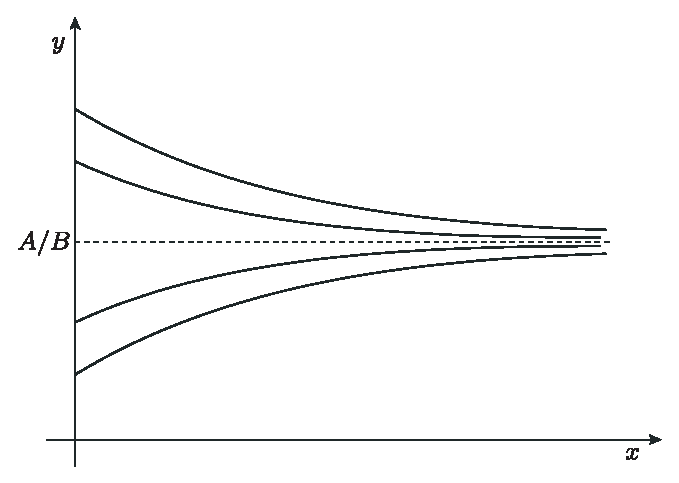
\includegraphics[width=11cm]{SL_212}
  %\fxnote{x umjesto t na slici}
\end{center}

\end{rj}
